\chapter{Selección de Componentes}

\section{Objetivo}
			Se estudiaron los componentes del proyecto y sus diversas alternativas de implementación por medio de un análisis comparativo que permitió evidenciar
			las características relevantes de cada uno de ellas. Inicialmente se realizó una comparativa de las prestaciones de los microprocesadores softcore
			más importantes para evaluar su capacidad de procesamiento.

\section{Selección del Microprocesador Soft-Core}


En la elección de los microprocesadores Soft-Core presentados en el capitulo anterior nos basamos principalmente en el requerimiento de usuario sobre el Hardware que nos requería implementar un Microprocesador Soft-core que prestara un rendimiento igual o superior a sus competidores comerciales. Tras la evaluación de las ventajas y desventajas se determinó el uso del microprocesador OpenRISC 1200. 	

		    			
\section{Presentación de SoCs basados en OpenRISC}
				
				\subsection{Proyecto MinSoC}
				La implementación llamada Minimal OpenRISC System on Chip utiliza IP cores estándar disponibles en OpenCores. Agrupa los cores necesarios para un SoC utilizando el procesador softcore OpenRISC OR1200. Este SoC puede sintetizarse para cualquier FPGA y placa de desarrollo sin necesidad de realizar cambios en su descripción RTL. Para cumplir con esta premisa el proyecto se basa en una implementación básica de memoria y posee una unidad de debug llamada Advanced Debug System, que permite depurar el sistema y cargar los programas a ejecutar con la misma interfase utilizada para la configuración de la FPGA.		

El proyecto brinda soporte nativo a diversas placas y FPGAs mediante definiciones en el código RTL y constraint files.
				pero puede adaptarse a otras siguiendo una mínima serie de pasos. Se cuenta además con una serie testbenchs y firmwares que permiten realizar
				pruebas funcionales del sistema y sirven de guía en los primeros desarrollos. Esta serie de testbenchs pueden ser ejecutados mediante la
				aplicación Icarus Verilog v.9.1 disponible en los repositorios estándar de la mayoría de las distribuciones Linux. 
				
				Existe una instancia de memoria on-chip de tamaño adaptable necesaria para soportar el firmware del CPU, que conjuntamente con los cores que
				soportan los periféricos básicos se adaptan de acuerdo a las capacidades de la FPGA destino. 

Una visión general sobre el SoC completa y sus conexiones externas se observa en la figura~\ref{fig:esquemaminsoc}

\begin{figure}[h!]
 \begin{center}
  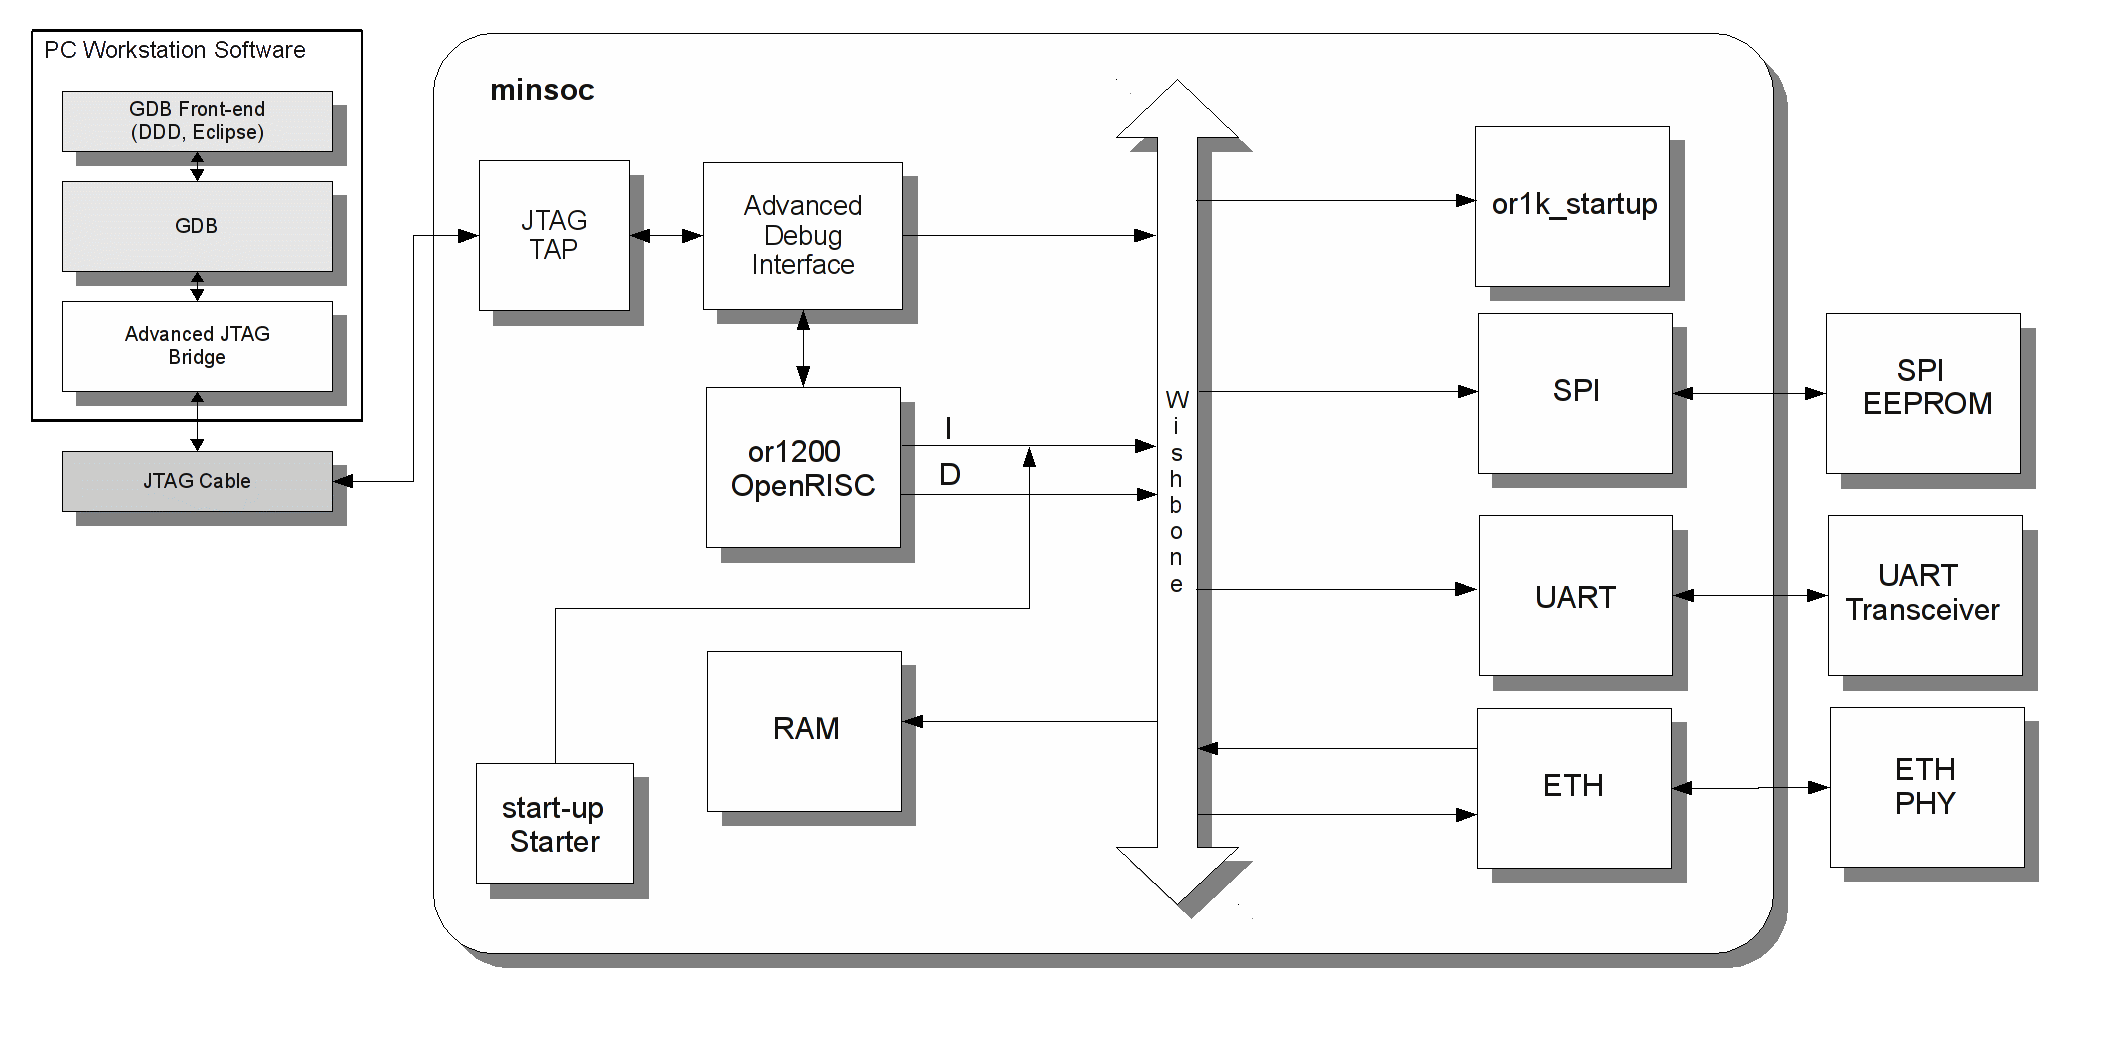
\includegraphics[width=1\textwidth,keepaspectratio=true]{./images/minsoc}
  \caption{Arquitectura MinSoC}
  \label{fig:esquemaminsoc}
 \end{center}
\end{figure}

\begin{itemize}
\item Características:
				\begin{itemize}
				  \item Microprocesador embebido OR1200 OpenRISC 
				  \item memoria redimensionalble
				  \item selección de frecuencia del sistema
				  \item JTAG debug 
				  \item Posibilitad de arranque automático de un firmware desde una memoria externa SPI
				  \item Modulos de UART y Ethernet 
				  \item Código genérico y especifico de memoria para las FPGA de Xilinx y Altera, adaptación de clock (PLLs y MCMs) y JTAG TAP
				  \item Configuración del sistema en un simple archivo de definición 
				  \item Ejemplos de firmware utilizando UART y Ethernet  
				  \item Incluye testbench para la simulacón de la configuración del sistema						
				\end{itemize}

\item Tecnologías probadas que le brindan soporte al proyecto MinSoC:


\begin{itemize}
				  \item Xilinx, Spartan 3E (Spartan3E Starter Kit)
				  \item Xilinx, Spartan 3A (Spartan3A 1800 DSP Kit)
				  \item Xilinx, Virtex 4 (ML405 board)
				  \item Xilinx, Virtex 5 (ML505 board)
				  \item Altera, Cyclone II
				  \item Altera, Cyclone II
				  \item (DE2-70 board)
				  \item Altera, Cyclone III
				  \item Altera, Cyclone IV (Bemicro SDK board) 
				  \item Altera, Stratix II						
				\end{itemize}
\end{itemize}

%\newpage
				\subsection{Proyecto ORPSoC}

				Este proyecto implementa una plataforma para el desarrollo OpenRISC. Está destinado a ser un entorno de desarrollo y verificación de IP cores y
				diseños de SoC. Se trata de un proyecto desarrollado con la colaboración de una de las comunidades mas importantes de hardware de código abierto
				\url{opencores.org}.


El proyecto permite tanto a usuarios nuevos como experimentados realizar diseños con un desarrollo rápido OpenRISC. Está destinado a ser un entorno de desarrollo y verificación de núcleos de propiedad intelectual y diseños SoC. Es un proyecto de desarrollo colaborativo. Como plataforma de desarrollo proporciona un entorno modular y fácil de usar, para el desarrollo de código RTL y su posterior simulación y síntesis. Provee un entorno de herramientas para desarrollo de aplicaciones OpenRISC para su simulación y prueba en la placa de desarrollo.

Una visión general sobre el SoC completa y sus conexiones externas es en la  figura~\ref{fig:esquemaorpsoc}

\begin{figure}[h!]
 \begin{center}
  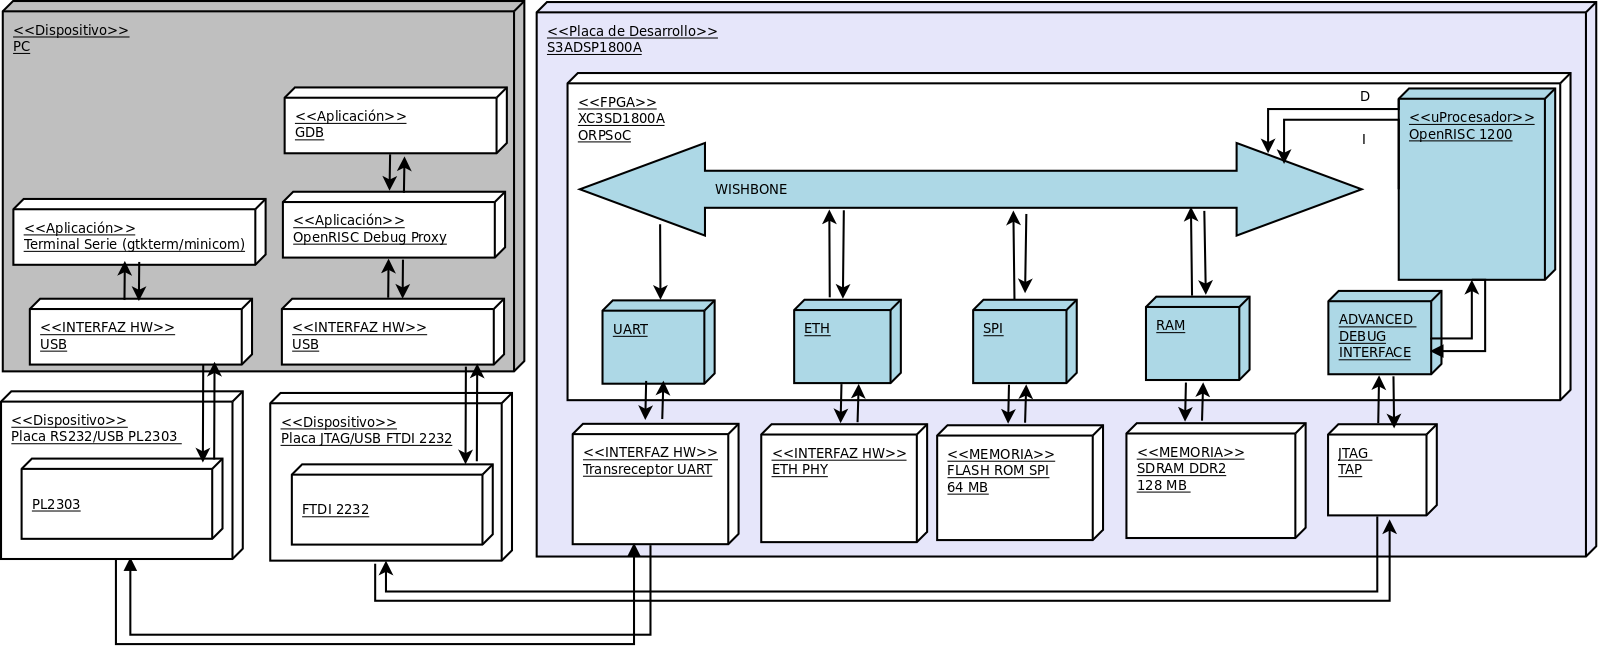
\includegraphics[width=1\textwidth,keepaspectratio=true]{./images/orpsoc}
  \caption{Arquitectura ORPsoc}
  \label{fig:esquemaorpsoc}
 \end{center}
\end{figure}

\begin{itemize}
\item Características:
				\begin{itemize}
				  \item Microprocesador embebido OR1200 OpenRISC 
				  \item memoria redimensionalble
				  \item selección de frecuencia del sistema
				  \item JTAG debug 
				  \item Posibilitad de arranque automático de un firmware desde una memoria externa SPI
				  \item Modulos de UART y Ethernet 
				  \item Código genérico y específico de memoria para las FPGA de Xilinx y Altera, adaptación de clock (PLLs y MCMs) y JTAG TAP
				  \item Configuración del sistema en un simple archivo de definición 
				  \item Ejemplos de firmware utilizando UART y Ethernet  
				  \item Incluye testbench para la simulacón de la configuración del sistema. 						
				\end{itemize}

\item Tecnologías probadas que le brindan soporte al proyecto MinSoC:


\begin{itemize}
				%  \item Xilinx, Spartan 3E (Spartan3E Starter Kit)
				  \item Xilinx, Spartan 3A (Spartan3A 1800 DSP Kit)
				  %\item Xilinx, Spartan 6 LX45 (ML405 board)
				  \item Xilinx, Virtex 5 (ML501 board
					% \item Altera, Cyclone II
				  %\item Altera, Cyclone II
				  %\item (DE2-70 board)
				%  \item Altera, Cyclone III
				  \item Altera, Cyclone IV (Terasic DE0 Nano) 
				%  \item Altera, Stratix II						
				\end{itemize}
\end{itemize}

				

\section{Presentación de Placas de Desarrollo}
 
				Los proyectos MinSoC y OrpSoc cuentan actualmente con soporte para diversas placas de desarrollo. 

				\subsection{Xilinx}
				La empresa Xilinx provee kits de desarrollo de diversas características y prestaciones. A continuación se detallan algunas de las alternativas soportadas por los SoC elegidos.
				\subsubsection{S3ADSP1800A}
				El dispositivo XtremeDSP™ Starter Platform cuenta con una FPGA de la familia Spartan®-3A que permite la evaluación diseños para diferentes
				aplicaciones tales como Prototipado General, Sistemas Embebidos, Video Digital, DSP, Procesamiento de Imágenes, Comunicaciones digitales y
				Coprocesamiento. Esta plataforma provee acceso a las capacidades de la familia de FPGA Spartan®-3A y cuenta con periféricos,conectores e
				interfaces estándar de la industria. Fue diseñada para para utilizarse con Xilinx System Generator para aplicaciones DSP y las herramientas de
				diseño ISE® o el entorno desarrollado en Linux llamado Peta Linux Software Development Kit (SDK), ambas herramientas provistas por el fabricante. 
				
				%Traducir esto ???
				Las características generales del kit son:
			
				\begin {table} [!h]
				\begin{tabular}{ p{4cm} p{10cm} }
				\rowcolor[gray]{0.8} Caracteristica & Descripción \\		
				\hline FPGA   & XC3SD1800A-4FGG676C Spartan-3A DSP FPGA\\
				\hline Clocks & 125 MHz LVTTL SMT oscillator\\
				\hline        & LVTTL oscillator socket\\
				\hline		  & 25.175 MHz LVTTL SMT oscillator (video clock)\\
				\hline		  & 25 MHz Ethernet clock (accessible to FPGA)\\
				\hline Memory & 128 MB (32M x 32) DDR2 SDRAM\\
				\hline		  & 16Mx8 parallel / BPI configuration flash\\
				\hline 		  & 64 Mb SPI configuration / storage flash (with 4 extra SPI selects)\\
				\hline Interfaces & 10/100/1000 PHY\\
				\hline			  & JTAG programming/configuration port\\
				\hline            & RS232 Port\\
				\hline			  & Low-cost VGA\\
				\hline			  & 4 SPI select lines\\
				\hline Buttons and Switches & 8 user LEDs\\
				\hline  		  & 8-position user DIP switch\\
				\hline            & 4 user push button switches\\
				\hline 			  & Reset push button switch\\
				\hline User I/O and Expansion & Digilent 6-pin header\\
				\hline			 			  & EXP expansion connector\\
				\hline 						  & 30-pin GPIO connector: can be used for System ACE™ Compact Flash daughter card (not included)\\
				\hline Configuration and Debug & JTAG\\
				\hline                         & System ACE module connector\\   
				\end{tabular}
				\caption {Características generales del kit de desarrollo S3ADSP1800A}
				\end {table}
				
				Las implementaciones MinSoC y ORPSoC proveen soporte nativo para los siguientes periféricos:
				
				\begin{itemize}
				  \item Ethernet
				  \item GPIO (Solo ORPSoC)
				  \item DDR2 SDRAM (128MB) (Solo ORPSoC)
				  \item SPI
				  \item UART				
				\end{itemize}
			
				\subsubsection{ML501}
				ML501 es una plataforma de desarrollo de bajo costo y gran funcionalidad que provee un acceso práctico a los recursos disponibles en el
				dispositivo FPGA Virtex®-5 LX50. Posee interfases y conectores industriales estándar y presenta gran versatilidad para su utilización en
				múltiples aplicaciones como Video, Audio y puertos de comunicación.
				
				Las características generales del kit son:
			
			\begin {table} [!h]
			\begin{tabular}{ p{4cm} p{10cm} }
			\rowcolor[gray]{0.8} Caracteristica & Descripción \\		
			\hline FPGA & XC5VLX50FFG676\\
			\hline Memoria & DDR2 SODIMM (256 MB)\\
			\hline 		   & ZBT SRAM (1 MB)\\
			\hline 		   & Linear Flash (32 MB)\\
			\hline         & System ACE™ CF technology (Compact Flash)\\
			\hline         & Platform Flash\\
			\hline         & SPI Flash\\
			\hline Clocks  & External clocking (2 differential pairs)\\
			\hline Interfaces & USB (2) - host and peripheral\\
			\hline 			  & PS/2 (2) - keyboard, mouse\\
			\hline 			  & RJ-45 - 10/100 Networking\\
			\hline 			  & RS-232 (male) - serial port\\
			\hline 			  & Audio In (2) - line, microphone\\
			\hline 			  & Audio Out (2) - line, amp, SPDIF, piezo speaker\\
			\hline 			  & Video (DVI/VGA) Output\\
			\hline I/O y expansión & Single-ended and differential I/O expansion\\
			\hline GPIO		&  DIP switch (8)\\
			\hline 			&  LEDs (8)\\
			\hline 			&  push buttons (5)\\
			\hline Debug y programación & JTAG programming interface\\
			\hline Medioambiente & EU-RoHS compliant \\
			\end{tabular}
			\caption {Características generales del kit de desarrollo ML501}	
			\end{table}
\newpage				
				Se probó la implementación ORPSoC en esta plataforma con éxito la plataforma y provee soporte para los siguientes periféricos:
				
				\begin{itemize}
				  \item Ethernet
				  \item GPIO
				  \item DDR2 SDRAM (256MB)
				  \item CFI flash (32MB)
				  \item SRAM
				  \item SPI
				  \item UART
				  \item AC97 
				  \item PS/2 				
				\end{itemize}
			
				
				\subsection{Digilent}
				\subsubsection{Atlys}
				La placa de desarrollo Atlys es una plataforma que permite el desarrollo de circuitos digitales y esta soportada por una FPGA Xilinx Spartan 6 LX45. Posee periféricos entre los que se destacan Gbit Ethernet, Video HDMI, Audio, puertos USB y Memoria Ram 128 MB DDR2 que permiten el
				desarrollo de Sistemas Digitales sobre procesadores embebidos como  MicroBlaze de Xilinx. Atlys es compatible con todas las herramientas CAD de
				Xilinx como ChipScope, EDK y WebPack (gratuito) lo que permite completar diseños sin mayor costo. Como alternativa puede utilizarse un entorno de
				desarrollo para Linux llamado PetaLinux Software Development Kit (SDK) provisto por el fabricante de la FPGA.
				
				Las características generales de la plataforma son:
				
				\begin {table} [!h]
				\begin{tabular}{ p{4cm} p{10cm} }
				\rowcolor[gray]{0.8} Caracteristica & Descripción \\		
				\hline FPGA   & Spartan-6 LX45, 324-pin BGA package \\
				\hline 		  &	6,822 slices each containing four 6-input LUTs and eight flip-flops\\
				\hline DSP	  & 58 DSP slices\\
				\hline Clocks & 2.1Mbits of fast block RAM\\
				\hline 		  & 4 clock tiles (8 DCMs \& 4 PLLs)\\
				\hline 		  & 6 phased-locked loops\\
				\hline 		  & 500MHz+ clock speeds\\
				\hline 		  & 100MHz CMOS oscillator\\
				\hline Memoria & 128Mbyte DDR2 16-bit wide data\\
				\hline         & 16Mbyte x4 SPI Flash for configuration \& data storage\\
				\hline GPIO & 8 LEDs \\
				\hline 		& 6 buttons\\
				\hline		& 8 slide switches\\
				\hline Interfaces & 10/100/1000 Ethernet PHY\\
				\hline 			  & On-board USB2 ports for programming \& data transfer\\
				\hline 			  & USB-UART and USB-HID port (for mouse/keyboard)\\
				\hline 			  & Two HDMI video input ports \& two HDMI output ports\\
				\hline			  & AC-97 Codec with line-in, line-out, mic, \& headphone\\
				\hline Energía & Real time power monitors on all power rails\\
				\hline 		   & 20W power supply and USB cable\\
				\hline I/O y Expansión & 48 I/O’s routed to expansion connectors\\
				\end{tabular}
				\caption{Características generales del kit de desarrolo Atlys}
				\end{table}
				La implementación ORPSoC proveen soporte nativo para los siguientes periféricos:
				
				\begin{itemize}
				  \item AC97
				  \item Ethernet
				  \item GPIO
				  \item PS/2 
				  \item DDR2 SDRAM (128MB)
				  \item SPI
				  \item UART
				  \item VGA
				\end{itemize}				

				\subsection{Terasic}
				\subsubsection{Terasic DE0 Nano}
				La plataforma DE0-Nano posee un tamaño compacto que se ajusta al diseño de circuitos para proyectos portables. Fue diseñada como una implementación simple utilizando como destino una FPGA Cyclone IV de Altera con 22,320 LEs (Elementos Lógicos). Entre sus
				características princpiales se encuentran diversas interfases que incluyen dos puertos de expanxión GPIO, dispositivos de memoria onboard SDRAM y
				EEPROM. Las mayores ventajas del DE0-Nano son su reducido tamaño y peso, así como la capacidad de ser reconfigurado sin la necesidad de
				utilización de hardware extra. Los requerimientos de energía para dispositivos portables son cruciales , la DE-0 Nano posee 3 esquemas posibles
				de conexión : un puerto USB mini-AB, conectores de 2 pines para alimentación externa de 5V, y 2 pines de 5V.

				Las características generales de la plataforma son:
				
				\begin{table} [!h]
				\begin{tabular}{ p{4cm} p{10cm} }
				\rowcolor[gray]{0.8} Caracteristica & Descripción \\		
				\hline FPGA   	& Cyclone® IV EP4CE22F17C6N FPGA\\
				\hline 			& 22,320 Logic elements (LEs)\\
				\hline 			& 594 Embedded memory (Kbits)\\
				\hline 			& 66 Embedded 18 x 18 multipliers\\
				\hline			& 4 General-purpose PLLs\\
				\hline 			& 153 Maximum FPGA I/O pins\\ 
				\hline Configuration Status and Set-Up Elements & 	On-board USB-Blaster circuit for programming\\
				\hline											&	FPGA Serial Configuration Device (EPCS)\\
				\hline Expansion Header & 	Two 40-pin Headers (GPIOs) provides 72 I/O pins\\
				\hline 					&	Two 5V power pins, two 3.3V power pins and four ground pins\\
				\hline 					&	One 26-pin header provides 16 digital I/O pins and 8 analog input pins to connect to analog sensors, etc\\ 
				\hline Memory Devices	&	32MB SDRAM\\
				\hline 					&	2Kb I2C EEPROM\\ 
				\hline General User Input/Output 	& 8 green LEDs\\
				\hline 								& 2 debounced push-buttons\\
				\hline 								& 4 dip switches\\ 
				\hline G-Sensor & ADI ADXL345, 3-axis accelerometer with high resolution (13-bit)\\ 
				\hline A/D Converter & NS ADC128S022, 8-Channel, 12-bit A/D Converter\\ 
				\hline					 & 50 ksps to 200 ksps \\
				\hline Clock System & On-board 50MHz clock oscillator\\
				\hline Power Supply & USB Type mini-AB port (5V)\\
				\hline 				& Two DC 5V pins of the GPIO headers (5V)\\
				\hline 				& 2-pin external power header (3.6-5.7V)\\
				\end{tabular}
				\caption {Características generales del kit de desarrollo DE0 Nano }
				\end{table}
				
				La implementación ORPSoC proveen soporte nativo para los siguientes periféricos:
				
				\begin{itemize}
				  	\item GPIO
					\item SDRAM (32MB)
					\item UART
					\item SPI FLASH (8MB)
					\item I2C
				\end{itemize}				
				
 		\subsection{Conclusiones de la elección de la placa de desarrollo}
 				Se seleccionó entre los items analizados y teniendo en cuenta la disponibilidad de recursos al momento de realizar este trabajo la
 				placa S3ADSP1800A de Xilinx para soportar los SoC a implementar.
 		
 		\newpage	
 		\section{Presentación de las Herramientas de Desarrollo} 	 
 				\subsection {Herramientas de desarrollo de hardware}
 				Durante el proceso de desarrollo e implementación de hardware mediante lógica programable son necesarias un serie de herramientas que
 				proporcionan diferentes salidas en cada etapa del proceso. En la Figura ~\ref{fig:designflow} se observan las etapas del flujo de diseño y sus
 				respectivas salidas.
 				
 		\begin{figure}[h!]
 		\begin{center}
  		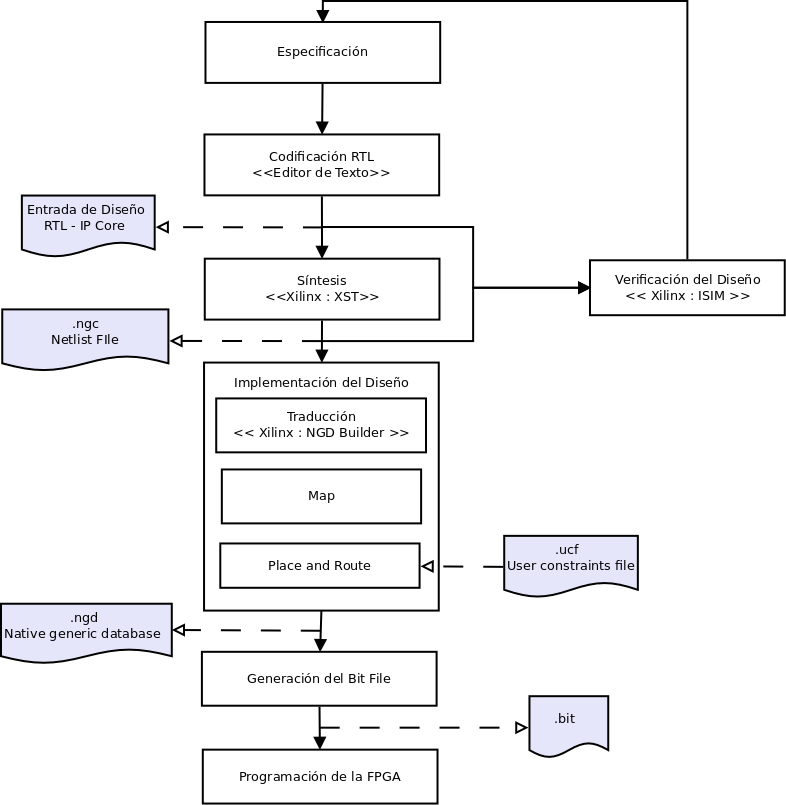
\includegraphics[width=0.7\textwidth,keepaspectratio=true]{./images/designflow}
  		\caption{Flujo de diseño e implementación de hardware con lógica programable}
  		\label{fig:designflow}
 		\end{center}
		\end{figure}
		
				Se analizaron las aplicaciones alternativas para cada etapa, enfatizando la selección de aplicaciones que cumplan con el requerimiento RQX-LC 2
				planteado en la Tabla ~\ref{tab:requsr2}.   
				
				\subsubsection {Codificación RTL - editores de texto}
				Existen diversas herramientas de Edición de Texto que poseen características compatibles con el desarrollo de código de descripción de hardware.
				Entre las características más comunes encontramos numeración de líneas, resaltado de código, y predictores. 
				Xilinx provee en su Suite de Desarrollo la posibilidad de confeccionar código directamente desde ISE Project Mananger. Sin embargo,
				existen alternativas Open Source de capacidades comparables tales como emacs o gedit. 
				
				\subsubsection {Síntesis, implementación del diseño y generación del Bit File}
				En estas etapas del proceso de diseño no existen herramientas alternativas con licencias OpenSource que permitan obtener el archivo de
				configuración de la FPGA. Esta restricción obliga a los desarrolladores a utilizar solo las herramientas del fabricante al implentar sus diseños
				en FPGA.
				Para realizar la síntesis, Xilinx, utiliza la aplicación XST que realiza la traducción de la descripción RTL escrita en algún lenguaje de
				descripción de Hardware como Verliog o VHDL en una lista de elementos lógicos y sus conexiones. La siguiente etapa consiste en la implementación 
				del diseño y consta de tres grandes etapas: Translate, Map, Place and Route. Finalizada esta etapa, se obtiene el diseño adecuado al modelo de FPGA seleccionado, sus clocks y sus conexiones de entrada/salida. 
				
				\subsubsection {Programación y configuración de la FPGA}
				La acción que culmina el proceso de implementación es la descarga del código binario de configuración en la FPGA. El protocolo utilizado para
				realizar esta acción se denomina JTAG (Joint Test Action Group) y se encuentra implementado en diversos dispositivos de programación de FPGA y
				microprocesadores. La mayoría de estos dispositivos proveen soporte SPI (Serial Peripheral Interface) que permite el acceso a dispositivos de
				almacenamiento como por ejemplo, las memorias Flash SPI.
				
				Xilinx provee la aplicación iMPACT con su Suite de Desarrollo ISE. Esta herramienta es compatible con todos los dispositivos fabricados por
				Xilinx y algunos dispositivos incluídos en sus placas de prueba. Durante el desarrollo de este trabajo los autores debieron lidiar con
				problemas de acceso a dispositivos de terceros que conforman la placa de desarrollo S3ADSP1800A que produjeron retrasos significativos en la
				realización del proyecto.
 				
 				Alternativamente, existen herramientas Open Source tales como XC3SPROG y UrJTAG, ambos licenciados bajo GPLv2. La herramienta XC3SPROG
 				posee capacidades comparables a iMPACT y proporciona acceso de diversos dispositivos entre los que se encuentran:
 				\begin{itemize}
 				  \item Dispositivos Xilinx
				  \item Dispositivos Atmel 
				  \item Memorias SPI flash: AT45, AMIC, AMIC-QUAD, M25P, N25Q, S33, W25
 				\end{itemize}
 				 
 				\subsection {Herramientas de desarrollo de software}
 			
				Se analizaron las aplicaciones alternativas para cada etapa, enfatizando la selección de aplicaciones que cumplan con el requerimiento RQX-LC 3
				planteado en la tabla ~\ref{tab:requsr2}.   
				 			
 				\subsubsection {Toolchain para OpenRISC}
 				La comunidad OpenCores realizó una adapatación del Toolchain GNU para generar aplicaciones en C y C++ que se ejecuten en una arquitectura
 				OpenRISC. Así mismo, se adaptaron las bibliotecas newlib y uClibc conformando una solución completa al diseño y desarrollo de aplicaciones
 				OpenRISC. Existe un entorno de desarrollo gráfico llamado OpenIDEA desarrollado por Dynalith basado en este toolchain. 
				
				El proyecto OpenRISC cuenta con un simulador del repertorio de instrucciones llamado \verb|or1ksim| que permite la simulación de aplicaciones compiladas
				mediante el toolchain sin necesidad de tener disponible el hardware de prueba durante la etapa de desarrollo de software.
 				
 	

		\section{Presentación de los Sistemas Operativos}
 		
			 	\subsection{ecOS}

eCos \cite{Etiqueta35} es un sistema operativo de tiempo real y de código abierto para aplicaciones embebidas, desarrollado por eCosCentric, una división de RedHat. Fue utilizado en varios productos como 
por ejemplo receptores de radio satelital Sirius, módulos Wi-Fi de la consola Sony PlayStation 3 
y routers Netgear, entre otros. 

 eCos viene de ``Embedded Configurable Operating System", y según sus creadores se puede configurar para ejecutarse tanto en dispositivos con memoria muy limitada de tipo SoC (System on a Chip) como en sistemas más complejos que requieren mayores funcionalidades. 
 
El sistema se distribuyo sin costo bajo licencia GPL modificada, la cual permite el uso de código propietario en conjunto con eCos. Esto significa que la licencia no requiere que el código desarrollado sobre eCos sea necesariamente de tipo GPL. También existe una versión comercial 
(eCosPro).

Características generales: 
				\begin{itemize}
				  	\item Algoritmo de iteración de tipo Round Robin
					\item Kernel de tipo apropiativo o cooperativo (configurable). Pueden añadirse schedulers 
 adicionales
					\item El Kernel no desactiva las interrupciones
					\item Implementación de mutexes, semáforos binarios y de conteo, variables de condición, 
 casillas de correo, banderas de evento y spinlocks
					\item Memory Allocation: Fixed Block, Variable Block y dynamic heaps. (configurable)
					\item Bibliotecas disponibles ISO C y Math, C++/STL, microITRON y POSIX. 
					\item  Incluye un pequeño stack IP
					\item Sistema de Archivos FAT12/16/32
					\item Incluye un bootloader con opciones de debugging
				\end{itemize}			

Arquitecturas compatibles:

				\begin{itemize}
				\item x86 / i386 / IA-32
				\item x86 Multiprocesamiento simétrico
				\item x86-64
				\item PowerPC Multiprocesamiento simétrico
				\item Alpha
				\item ARM
				\item Intel XScale
				\item M68k
				\item PA-RISC
				\item OpenRISC
				\item CalmRISC
				\item Nios II
			\end{itemize}			

			 \subsection{Linux}

El sistema operativo Linux es una implementación de libre distribución de tipo UNIX para computadoras personales (PC), servidores, y estaciones de trabajo. EL sistema operativo Linux tiene un kernel eficiente.

 
Características generales:

	\begin{itemize}
	\item Licencia de Software: GPL/LGPL
	\item Tipo de núcleo: núcleo monolítico con módulo
	\item Lenguaje de programación del núcleo en c
	\item Soporte de Hilos de ejecución del núcleo: 1:1
	\item Familia de SO tipo UNIX
	\item Comunicación entre procesos y sincronización
	\item Multitarea
	\item Unidad de Gestión de Memoria 
	\item Tecnología de red TCP/IP,IPv6, IPX, PPP, PPPoE, DHCP, bridge, TUN/TAP, ssh, OpenVPN 	
	\item Sistema de archivos NTFS,ext2, MS-DOS, FAT16/32 y otros
	\item Forks: microCLinux	
	
\end{itemize}			

Arquitecturas compatibles:

				\begin{itemize}
				\item x86 / i386 / IA-32
				\item x86 Multiprocesamiento simétrico
				\item Xen
				\item IA-64 	
				\item SPARC32
				\item x86-64
				\item PowerPC
				\item PowerPC Multiprocesamiento simétrico
				\item Alpha
				\item MIPS
				\item ARM
				\item Intel XScale
				\item M68k
				\item PA-RISC
				\item OpenRISC
			\end{itemize}			


		\subsection{BusyBox}	
 	
				
			 
BusyBox \cite{Etiqueta36} combina versiones de varias utilidades comunes de UNIX en un sólo ejecutable. Remplaza las utilidades que se suelen encontrar en fileutils GNU, shellutils, etc. %Las utilidades en BusyBox tienen menos funciones que GNU, sin embargo, las opciones que incluyen proporcionan la funcionalidades necesarias.
BusyBox proporciona un entorno  completo para cualquier sistema pequeño o embebido.

Este conjunto de programas están optimizados de acuerdo a las limitaciones de los recursos disponibles de hardware. También se puede fácilmente incluir o excluir comandos (o características) en tiempo de compilación. Esto hace que sea fácil de personalizar un sistemas embebidos. 

%Para crear un sistema de trabajo, sólo tiene que añadir algunos nodos de dispositivos en / dev, algunos archivos de configuración en / etc, y un núcleo de Linux.

BusyBox tiene licencia GNU GPL y lo mantiene Denys Vlasenko.
%%%%%%%%%%%%%%%%%%%%%%%%%%%

			
 			
 
